\documentclass{beamer}
\setbeamertemplate{navigation symbols}{}
\setbeamertemplate{bibliography item}[text]

\usepackage{beamerthemeshadow}
\usepackage{amsmath}
\usepackage{amssymb}
\usepackage{graphicx}
\graphicspath{ {./images/} }
\begin{document}
\title{Perfect graphs: definition, examples, characterizations}  
\author{Coman Florin-Alexandru}

\begin{frame}
\titlepage
\end{frame}

\begin{frame}\frametitle{Table of contents}\tableofcontents
\end{frame}

\section{Definitions}
\subsection{Perfect Graph}
\begin{frame}\frametitle{Perfect Graph}
\begin{block}{Definition}
A \textbf{perfect graph} is a graph $G$ such that for every induced subgraph of $G$, the clique number equals the chromatic number, i.e., $\omega(G) = \chi(G)$. A graph that is not a perfect graph is called an imperfect graph.
\end{block}
\end{frame}

\subsection{Weakly Perfect Graph}
\begin{frame}\frametitle{Weakly Perfect Graph}
\begin{block}{Definition}
A graph for which $\omega(G) = \chi(G)$ (without any requirement that this condition also hold on induced subgraphs) is called a \textbf{weakly perfect graph}. All perfects graphs are therefore by definition weakly perfect.
\end{block}
\end{frame}

\subsection{Strongly Perfect Graph}
\begin{frame}\frametitle{Strongly Perfect Graph}
\begin{block}{Definition}
A graph is \textbf{strongly perfect} if every induced subgraph $H$ has an independent set meeting all maximal cliques of $H$. While all strongly perfect graphs are perfect, the converse is not necessarily true. Since every $P_4$-free graph (where $P_n$ is a path graph) is strongly perfect and every strongly perfect graph is perfect, if a graph is $P_4$-free, it is perfect.
\end{block}
\end{frame}

\section{Classes of graphs that are perfect}
\subsection{Bipartite Graphs}
\begin{frame}\frametitle{Bipartite Graphs}
\begin{block}{Definition}
A \textbf{bipartite graph}, also called a bigraph, is a set of graph vertices decomposed into two disjoint sets such that no two graph vertices within the same set are adjacent. A bipartite graph is a special case of a k-partite graph with $k=2$. \\
The illustration above shows some bipartite graphs, with vertices in each graph colored based on to which of the two disjoint sets they belong.
\end{block}
\begin{exampleblock}{Example}
\begin{figure}[h]
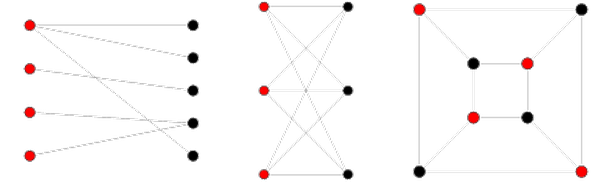
\includegraphics[width=5.5cm]{picture1}
\end{figure}
\end{exampleblock}
\end{frame}

\subsection{Chordal Graphs}
\begin{frame}\frametitle{Chordal Graphs}
\begin{block}{Definition}
A graph is called \textbf{chordal} if every cycle of length at least four contains a chord. These graphs are also called triangulated.
\end{block}
\begin{exampleblock}{Example}
\begin{figure}[h]
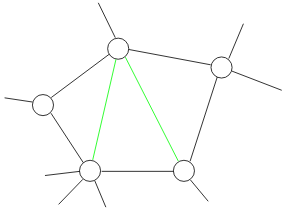
\includegraphics[width=4cm]{picture2}
\end{figure}
A cycle (black) with two chords (green).
\end{exampleblock}
\end{frame}

\subsection{Interval Graphs}
\begin{frame}\frametitle{}
\begin{block}{Definition}
A graph is an \textbf{interval graph} if each vertex can be represented by an interval on the real line in such a way that two vertices are adjacent if and only if their corresponding intervals intersect. These graphs are $\longrightarrow$ triangulated and therefore perfect.
\end{block}
\begin{exampleblock}{Example}
\begin{figure}[h]
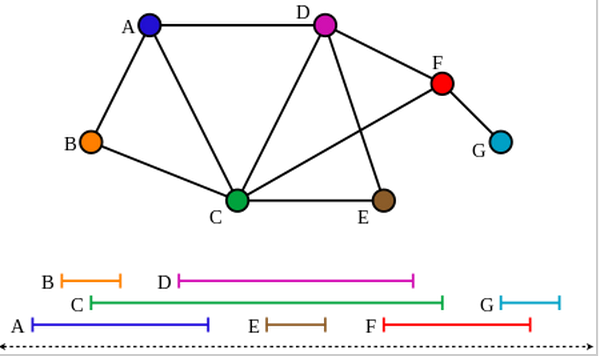
\includegraphics[width=5.5cm]{picture4}
\end{figure}
\fontsize{8.5pt}{7.2}\selectfont
Seven intervals on the real line and the corresponding seven-vertex interval graph.
\end{exampleblock}
\end{frame}

\subsection{Split Graphs}
\begin{frame}\frametitle{Split Graphs}
\begin{block}{Definition}
A graph is called split if its vertex set can be partitioned into two sets $V_1$ and $V_2$ such that $V_1$ induces a stable set and $V_2$ induces a clique. Perfection of split graphs follows from the fact that they are triangulated.
\end{block}
\begin{exampleblock}{Example}
\begin{figure}[h]
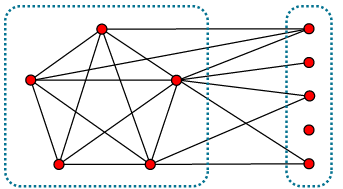
\includegraphics[width=5.5cm]{picture3}
\end{figure}
\end{exampleblock}
\end{frame}

\section{Characterizations}
\subsection{Strong Perfect Graph Theorem}
\begin{frame}\frametitle{Strong Perfect Graph Theorem}
\begin{block}{}
The theorem, originally conjectured by Berge (1960, 1961), that a graph is perfect iff neither the graph nor its graph complement contains an odd graph cycle of length at least five as an induced subgraph became known as the strong perfect graph conjecture (Golumbic 1980; Skiena 1990, p. 221). The conjecture can be stated more simply as the assertion that a graph is perfect iff it contains no odd graph hole and no odd graph antihole. The proposition can be stated even more succinctly as "a graph is perfect iff it is a Berge graph."
\end{block}
\end{frame}

\section{Bibliography}
\begin{frame}[allowframebreaks]
\frametitle{Bibliography}
    \tiny{\bibliographystyle{abbrv} }
    \bibliography{main}
\end{frame}

\end{document}